\section{ElasticSearch}
\par Elasticsearch是一个开源分布式搜索引擎,可以看作一个分布式Key-Value数据库,它的特点有:分布式,零配置,自动发现,索引自动分片,索引副本机制,Restful风格接口,多数据源,自动搜索负载等。
\par Types are just syntactic sugar to add separation between types of documents. If you know Lucene, type is just a field on a doc。Lucene index has Documents and has no notion of types. Types are something added (as best as possible) by elasticsearch. A lucene document is a flat structure(一种扁平结构) key value pair (so objects in json are also translated to this), and a type ends up as another field within the document (called \_type),也就是说,type的值将赋给每个Document的\textbf{\_type}域。
\par 当index为cars,type为car时,ElasticSearch将自动为每个查询添加一个必须满足的条件(只有\textbf{\_type}域的值为car的Document才能匹配到查询),更新索引也是如此。This does mean that across types, having the same field name with different mappings types (for example, \textbf{'car'} has field \textbf{'Seat'} of type numeric, and 'bus' also has field \textbf{'Seat'} but of type string) should not be done (\textbf{car}和\textbf{bus}分别作为\textbf{type}的值). The type prefix when you define the field name should allow to only search on a field against that specific type.
\par Each document indexed is associated with an id and a type, the internal \_uid field is the unique identifier of a document within an index and is composed of the type and the id (meaning that different types can have the same id and still maintain uniqueness).ElasticSearch Index每个分片(实际上是一独立的Lucene Index)中,内部域只有两个(通过Document.getFields()函数获得,而MultiFields.getIndexedFields函数也可以获得多个域,现在还不清楚这两个函数什么区别),分别是\_uid和\_source。The \_uid field is automatically used when \_type is not indexed to perform type based filtering, and does not require the \_id to be indexed(注意Java类:src/main/java/org/elasticsearch/index/mapper/Uid.java).假如type为table,id为http://www.wuxi.gov.cn/zxzx/wxyw/6711554.shtml,则返回的\textbf{\_uid}为table\#http://www.wuxi.gov.cn/zxzx/wxyw/6711554.shtml,中间添加了一个\#号,因此ES不允许id值中出现\#这种字符。
\subsection{What's a mapping?}
\par A mapping tells ES what terms are indexed and searchable, is composed of one or more ‘analyzers’(相当于Lucene中的Analyzer), which are in turn built with one or more ‘filters’. When ES indexes your document, it passes the field into each specified analyzer, which pass the field to individual filters.
\par Filters are easy to understand: a filter is a function that transforms data. Given a string, it returns another string (after some modifications). An analyzer is simply a group of filters that are executed in-order. So an analyzer may first apply a lowercase filter, then apply a stop-word removal filter(中文分词也可作为其中一个filter)。 Once the analyzer is run, the remaining terms are indexed and stored in ES。因此, a mapping is simply a series of instructions on how to transform your input data into searchable, indexed terms.
\par 使用\textbf{curl -XPUT localhost:9200/test/item/1 -d '\{"name":"zach", "description": "A Pretty cool guy."\}'}时,ES生成如下的mapping:
\begin{verbatim}
mappings: {
   item: {
      properties: {
         description: { type: string }
         name: { type: string }
      }
   }
}
\end{verbatim}
\par ES猜测到"description"列的类型为"string",When ES implicitly creates a "string" mapping, it applies the default Standard Analyzer。除非显式地更改analyzer设置,否则ES将使用默认的Standard Analyzer。Standard Analyzer will apply the standard token filter, lowercase filter and stop token filter . 这种情况下,description列中的“.”号和字符“A”将被丢弃.Importantly, even though ES continues to store the original document in it’s original form, the only parts that are searchable are the parts that have been run through an analyzer.So, mappings are not data-types , think of them as instructions on how you will eventually search your data. If you care about stop-words like 'a', you need to change the analyzer so that they aren’t removed.
\par The first thing that happens to an input query is tokenization , breaking an input query into smaller chunks called tokens. There are several tokenizers available, which you should explore on your own when you get a chance. The Standard tokenizer is being used in this example, which is a pretty good tokenizer for most English-language search problems. You can query ES to see how it tokenizes a sample sentence:
\begin{verbatim}
curl -X GET "http://localhost:9200/test/_analyze?tokenizer=standard&pretty=true" 
-d 'The quick brown fox is jumping over the lazy dog.'
curl -X GET "http://localhost:9200/test/_analyze?filter=standard&pretty=true" 
-d 'The quick brown fox is jumping over the lazy dog.'
\end{verbatim}
\par As you can see, we specify both a search and index analyzer. These two separate analyzers instruct ES what to do when it is indexing a field, or searching a field. But why are these needed?
\begin{verbatim}
"partial":{
     "search_analyzer":"full_name",
     "index_analyzer":"partial_name",
     "type":"string"
}
\end{verbatim}
\par The index analyzer is easy to understand. We want to break up our input fields into various tokens so we can later search it. So we instruct ES to use the new partial\_name analyzer that we built, so that it can create nGrams for us.
\par The search analyzer is a little trickier to understand, but crucial to getting good relevance. Imagine querying for “Race”. We want that query to match “race”, “races” and “racecar”. When searching, we want to make sure ES eventually searches with the token “race”. The full\_name analyzer will give us the needed token to search with.
\par If, however, we used the partial\_name nGram analyzer, we would generate a list of nGrams as our search query. The search query “Race” would turn into ["ra", "rac", "race"].Those tokens are then used to search the index. As you might guess, “ra” and “rac” will match a lot of things you don’t want, such as “racket” or “ratify” or “rapport”.
\par So specifying different index and search analyzers is critical when working with things like ngrams. Make sure you always double check what you expect to query ES with…and what is actually being passed to ES。使用如下命令搜索:
\begin{verbatim}
curl -XPOST "http://namenode:9200/_search" -d'
{
    "query": {
      "match_all" : {}
    },
    "filter" : {
      "term" : { "director" : "Francis Ford Coppola"}
    }
}'
\end{verbatim}
没有任何结果,而使用
\begin{verbatim}
curl -XPOST "http://namenode:9200/_search" -d'
{
    "query": {
      "match_all" : {}
    },
    "filter" : {
      "term" : { "year" : "1962"}
    }
}'
\end{verbatim}
\par 却能输出结果,When we index a document with ElasticSearch it (simplified) does two things: it stores the original data untouched for later retrieval in the form of \_source and it indexes each JSON property into one or more fields in a Lucene index. During the indexing it processes each field according to how the field is mapped. If it isn't mapped , default mappings depending on the fields type (string, number etc) is used.
\par As we haven't supplied any mappings for our index, ElasticSearch uses the default mappings for the director field. This means that in the index the director fields value isn't \textbf{"Francis Ford Coppola"}. Instead it's something like \textbf{["francis", "ford", "coppola"]}. We can verify that by modifying our filter to instead match "francis" (or "ford" or "coppola").
\par 如果想精确匹配整个Text,必须修改Text的映射方式(mapping)。There are a number of ways to add mappings to ElasticSearch, through a HTTP request that creates by calling the \_mapping endpoint. Using this approach, we could fix the above issue by adding a mapping for the "director" field , to instruct ElasticSearch not to analyze (tokenize etc.) the field at all.
\begin{verbatim}
curl -X PUT namenode:9200/movies/movie/_mapping -d'
{
   "movie": {
      "properties": {
         "director": {
            "type": "string",
            "index": "not_analyzed" (不分析director域)
        }
      }
   }
}'
\end{verbatim}
\par 有时无法修改索引的mapping,最简单的办法是删除原先的并重建索引,但这种方法无法同时满足两种查询(精确匹配整个Text或仅仅匹配Text中的某个string),此时可以设置director域的类型为"multi\_field",也就是说,对文档中的同一个域可以生成多个别名(每个别名再索引一次)。
\begin{verbatim}
curl -XPUT "namenode:9200/movies/movie/_mapping" -d'
{
   "movie": {
      "properties": {
         "director": {
            "type": "multi_field",
            "fields": {
              "director": {"type": "string"},
              "original": {"type" : "string","index" : "not_analyzed"}
               (使用director.original访问这个域)
            }
         }
      }
   }
}'
\end{verbatim}

\subsection{Depth into ElasticSearch}
\par 如果想查看ElasticSearch中某些或某几个index的状态,使用命令:
\begin{verbatim}
curl -XGET '192.168.50.75:9200/_status?pretty'
curl -XGET '192.168.50.75:9200/official_mini/_status?pretty'
curl -XGET 'http://localhost:9200/sogou_spellcheck/_mapping?pretty'
\end{verbatim}
\par Indices created within the cluster can provide their own settings. For example, the following creates an index with memory based storage instead of the default file system based one (尚且不清楚常驻内存的index在文件系统中是否有备份),常驻内存的index必定耗费heap。
\begin{verbatim}
$ curl -XPUT localhost:9200/official_mini/ -d 'index.store.type:memory'
\end{verbatim}
\par 如果ES占用内存过多,则性能会急剧下降,此时可以修改Java虚拟机内存参数,ES默认的heap最大值为1024M。Elasticsearch comes with built in JAVA\_OPTS passed to the JVM started. The most important setting for that is the -Xmx to control the maximum allowed memory for the process, and -Xms to control the minimum allocated memory for the process (一般情况下,分配内存越多,性能越好)。 Most times it is better to ignore the default JAVA\_OPTS settings, and use the ES\_JAVA\_OPTS environment variable to set/change JVM settings。可以修改\textbf{elasticsearch.in.sh}文件中的两个环境变量:\textbf{ES\_MIN\_MEM} (默认值为256m)和\textbf{ES\_MAX\_MEM} (默认值为1024m)。
\subsubsection{ES集群设置}
\par This will print the number of open files the process can open on startup. Alternatively, you can retrieve the max\_file\_descriptors for each node using the Nodes Info API, with:\\
\textbf{curl -XGET 'namenode:9200/\_nodes/process?pretty=true'},下面是删除ES上名为jdbc的index的Restfule命令:\\
\textbf{curl -XDELETE 'http://namenode:9200/jdbc/'}
\par 配置文件在\textbf{\{\$ES\_HOME\}/config}文件夹下,\textbf{elasticsearch.yml}和\textbf{logging.yml},修改\textbf{elasticsearch.yml}文件中的cluster.name,当集群名称相同时,每个ES节点将会搜索它的伙伴节点,因此必须保证集群内每个节点的cluster.name相同,下面是关闭ES集群的Restful命令:
\begin{verbatim}
# 关闭集群内的某个ES节点'_local'
$ curl -XPOST 'http://namenode:9200/_cluster/nodes/_local/_shutdown'
# 关闭集群内的全部ES节点
$ curl -XPOST 'http://namenode:9200/_shutdown'
\end{verbatim}
\par 注意,如果一台机器上不止一个ES在运行,那么通过\textbf{./bin/elasticsearch}开启的ES的http\_address将会使用9200以上的接口(形如9201,9202,$\cdots$),而相应的transport\_address也递增(形如:9301,9302,$\cdots$),因此,为使用9200端口,可使用上述命令关闭其它ES进程,可通过conf目录下的log文件来查看某些端口是否被占用。\textbf{elasticsearch.yml}文件存在如下配置信息:
\begin{enumerate}[(1)]
\item node.master: true,node.data: true,允许节点存储数据,同时作为主节点;
\item node.master: true,node.data: false,节点不存储数据,但作为集群的协调者;
\item node.master: false,node.data: true,允许节点存储数据,但不作为主节点;
\item node.master: false,node.data: false,节点不存储数据,也不作为协调者,但作为搜索任务的一个承担者;
\item cluster.name: HadoopSearch, node.name: "ES-Slave-02",HadoopSearch必须相同,但node.name每个节点可以自由设置;
\end{enumerate}
如想将ES作为一个服务,需要从github上下载elasticsearch-servicewrapper,然后调用chkconfig,将其添加到/etc/rc[0$\sim$6].d/中。
\begin{verbatim}
curl -L https://github.com/elasticsearch/elasticsearch-servicewrapper/archive/master.zip > master.zip
unzip master.zip
cd elasticsearch-servicewrapper-master/
mv service /opt/elasticsearch/bin
/opt/elasticsearch/bin/service/elasticsearch install
## 如果想卸载该服务调用:
/opt/elasticsearch/bin/service/elasticsearch remove
## 如果想让ES开机启动
chkconfig elasticsearch on  
## 如果想现在开启ES服务
service elasticsearch start 
\end{verbatim}
配置完后,可通过\textsl{curl -X GET 'http://192.168.50.75:9200/\_cluster/nodes?pretty'}命令,查询集群下的节点信息。
\par 为连接hive与ES,运行hive后,在hive命令行内执行\textbf{add jar /opt/elasticsearch-hadoop-1.3.0/dist/elasticsearch-hadoop-1.3.0.jar;}或者hdfs上的jar包:\textbf{add jar hdfs://namenode:9000/elasticsearch-hadoop-1.3.0.jar}可加载elasticsearch-hadoop插件,使用该插件的具体操作如下:
\begin{verbatim}
DROP TABLE IF EXISTS artist_1;
CREATE EXTERNAL TABLE artists_1 (
  cardid STRING, date STRING, time STRING)
STORED BY 'org.elasticsearch.hadoop.hive.ESStorageHandler'
TBLPROPERTIES('es.resource' = 'liubo/artists/',
              'es.host' = '192.168.50.75',
              'es.mapping.names' = 'text:time'
);
-- 集群下应使用'192.168.50.75',而非'localhost'(es-hadoop的默认值)
-- insert data to Elasticsearch from another hive table
INSERT OVERWRITE TABLE artists_1
SELECT * FROM cable.temptable;
\end{verbatim}
\par 下面的代码是将Mysql中的表导入到ES中,建立名为jdbc的index,表名称为jiangsu。
\begin{verbatim}
curl -XPUT 'localhost:9200/_river/jiangsu/_meta' -d '{
    "type" : "jdbc",
    "jdbc" : {
        "driver" : "com.mysql.jdbc.Driver",
        "url" : "jdbc:mysql://192.168.50.75:3306/jsyx",
        "user" : "root",
        "password" : "123456",
        "sql" : "select * from jiangsu"
    },
    "index" : {
        "index" : "jdbc",
        "type" : "jiangsu"
    }
}'
\end{verbatim}
\subsubsection{ES性能优化}
\par 一个Elasticsearch节点会有多个线程池,但重要的是下面四个:
\begin{itemize}
\item 索引(index):主要是索引数据和删除数据操作(默认是cached类型);
\item 搜索(search):主要是获取,统计和搜索操作(默认是cached类型);
\item 批量操作(bulk):对索引的批量操作,尚且不清楚它是不是原子性的,如果是原子的,则放在MapReduce里是没有问题的;
\item 更新(refresh):主要是更新操作,如当一个文档被索引后,何时能够通过搜索看到该文档;
\end{itemize}
\par 在建立索引(index相当于数据库,type相当于数据库中的表)的过程中,需要修改如下配置参数:
\begin{itemize}
\item index.store.type: mmapfs.因为内存映射文件机制能更好地利用OS缓存;
\item indices.memory.index\_buffer\_size: 30\% 默认值为10\%,表示10\%的内存作为indexing buffer;
\item index.translog.flush\_threshold\_ops: 50000,当写日志数达到50000时,做一次同步;
\item index.refresh\_interval:30s,默认值为1s,新建的索引记录将在1秒钟后查询到;
\end{itemize}
\begin{verbatim}
curl -XPUT 'http://namenode:9200/hivetest/?pretty' -d '{
    "settings" : {
       "index" : {
       "refresh_interval" : "30s",
       "index.store.type": "mmapfs",
       "indices.memory.index_buffer_size": "30%",
       "index.translog.flush_threshold_ops": "50000"
        }
    }
}'
\end{verbatim}
\par 但上述设置性能低下,也不知why?ES索引的过程相对Lucene的索引过程多了分布式数据的扩展,而ES主要是用tranlog进行各节点间的数据平衡,因此设置"index.translog.flush\_threshold\_ops"为"100000",意思是当tranlog数据达到多少条进行一次平衡操作,默认为5000,而这个过程相对而言是比较浪费资源的,必要时可以将这个值设为-1关闭,进而手动进行tranlog平衡。"refresh\_interval"是刷新频率,设置为30s是指索引在生命周期内定时刷新,一但有数据进来就在Lucene里面commit,因此其值设置大些可以提高索引效率。另外,如果有副本存在,数据也会马上同步到副本中去,因此在索引过程中,将副本设为0,待索引完成后将副本个数改回来。
\begin{verbatim}
curl -XPUT 'namenode:9200/hivetest/' #新建一个名为hivetest的索引
curl -XPOST 'namenode:9200/hivetest/_close' #关闭索引,为修改参数做准备
curl -XPUT 'namenode:9200/hivetest/_settings?pretty' -d '{
   "index" : {
      "refresh_interval" : "30s",
      "index.translog.flush_threshold_ops": "100000",
      "number_of_replicas" : 0
   }
}'
curl -XPOST 'namenode:9200/hivetest/_open'
\end{verbatim}
\par Linux主机上硬盘空间有限,经常发现root目录下已没有可利用磁盘空间,为此,将ES的日志和数据输出目录设置在/home目录下,修改config目录下的elasticsearch.yml文件中的选项,其中path.data为索引文件存放目录,path.work为临时文件存放目录,path.logs为日志文件存放目录。
\begin{verbatim}
path.data: /home/elasticSearch/data
path.work: /home/elasticSearch/work
path.logs: /home/elasticSearch/logs
\end{verbatim}
\subsection{Lucene索引}
\subsubsection{Lucene结构}
Lucene基础架构如图\ref{fig-lucene-1}示,
\begin{figure}[htbp]
\centering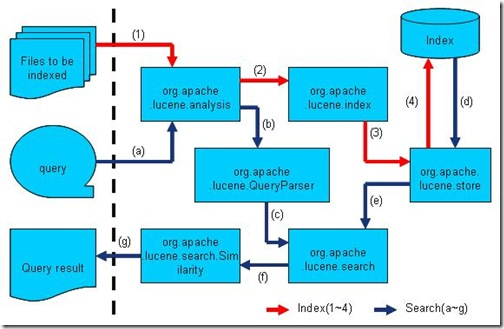
\includegraphics[width=.7\linewidth]{figures/lucene-architect.jpg}
\caption{Lucene基础架构图}\label{fig-lucene-1}
\end{figure} 
\begin{enumerate}[(1)]
\item Lucene的analysis模块主要负责词法分析及语言处理而形成Term。
\item Lucene的index模块主要负责索引的创建,里面有IndexWriter。
\item Lucene的store模块主要负责索引的读写。
\item Lucene的QueryParser主要负责语法分析。
\item Lucene的search模块主要负责对索引的搜索。
\item Lucene的similarity模块主要负责计算相关性。
\end{enumerate}
\par Lucene包含如下几种类型文件:
\begin{description}
\item [.tim]用于存放Term的库,contains the list of terms in each field along with per-term statistics (such as docfreq) and pointers to the frequencies, positions, payload and skip data in the .doc, .pos, and .pay files.
\item [.doc]Frequencies and Skip Data,估计用于计算文档相关性,contains the lists of documents which contain each term, along with the frequency of the term in that document.
\item [.pos]Positions,存储Term位置的文件,contains the lists of positions that each term occurs at within documents,此外,还有.tip类型文件(用于索引Term)和.pay类型文件(做什么,暂时不详)。
\end{description}
\par Lucene包含如下几种jar包:
\begin{enumerate}[(1)]
\item org.apache.lucene.util,一些公用基础设施。
\item org.apache.lucene.analysis,语言分析器,主要用于切分单词(英文根据空格),对中文的扩展支持可改写此类。
\item org.apache.lucene.document,索引存储时的文档结构管理,类似于关系型数据库的关系。
\item org.apache.lucene.index,索引管理,包括索引建立、删除,更新等。
\item org.apache.lucene.queryParser,查询分析器,实现查询关键词间的运算,如与、或、非等,据说写得十分复杂。
\item org.apache.lucene.search,检索管理,根据查询条件,检索得到结果。
\item org.apache.lucene.store,数据存储管理,包括一些底层I/O操作。
\end{enumerate}
\subsubsection{Lucene分词过程}
\par Analyzer类是所有分词器的基类,它是个抽象类,所有的子类必须实现它。它的功能实质上是将输入文本转化为文本特征向量,这里所说的文本特征,可以是词或者是短语,它主要包括四个步骤:(1)分词,将文本解析为单词或短语;(2)归一化,将文本转化为小写;(3)停用词处理,去除一些常用的、无意义的词;(4)提取词干,解决单复数、时态语态等问题。
\par Lucene Analyzer包含两个核心组件,Tokenizer以及TokenFilter。两者的区别在于,前者在字符级别处理流(即前者将字符串转换成Term),而后者则在词语级别处理流(对Term进行转换)。Tokenizer是Analyzer的第一步,其构造函数接收一个Reader(例如BufferedReader)作为参数,而TokenFilter则类似一个拦截器,其参数可以是TokenStream、Tokenizer,甚至是另一个TokenFilter。
\begin{description}
\item [Token]表示文中出现的一个词,它包含了词在文本中的位置信息等等;
\item [Analyzer]将文本转化为TokenStream的工具,Analyzer通过对文本的分析来建立TokenStream;
\item [TokenStream]由一个个Token组成的数据流,可以说Analyzer是一种从文本数据中抽取索引词(Term)的策略。
\item [Tokenizer]处理输入符号流,生成一个个Token;
\item [TokenFilter]处理符号流,输入可以是TokenStream,Tokenizer,TokenFilter;
\end{description}
\par Lucene提供了数十种内置的Tokenizer、TokenFilter以及Analyzer供开发人员使用,事实上大部分时候只需要使用其中几种,比如标准分词器StandardTokenizer、空格分词器WhitespaceTokenizer(按空格分词)、转化为小写格式的LowCaseFilter(将英文单词转换成小写)、提取词干的PoterStemFilter(提取英文词干,比如对英文的过去式,现在进行时等提取词干)以及组合使用StandardTokenizer和多种TokenFilter的StandardAnalyzer。 
\par 处理英文默认的Analyzer为StandardAnalyzer,当处理中文分词和拼音等特殊情况时,需要实现自定义的Analyzer,在处理汉字时最主要的工作是实现一个Tokenizer来分词,TokenFilter(汉字的停用词过滤等)不太复杂,可不做过多考虑。当继承Analyzer时,可override其提供的createComponents方法:
\begin{verbatim}
@Override
protected TokenStreamComponents createComponents(String fieldName,
        final Reader reader) {
    Tokenizer tokenizer = new SoulTokenizer(new BasicAnalysis(reader),
        reader, filter, pstemming);
    return new TokenStreamComponents(tokenizer);
}
\end{verbatim}
\par 上例中的fieldName没有用处,有两个类型的子类TokenFilter和Tokenizer(也可以继承CharTokenizer),Tokenizer通过读取汉字字符串创建词序列List<word>,其中每一word将作为Lucene索引的key,Tokenizer还记录每个word的偏移值,以及在文档中属于第几个word($0,\cdots,n$)等,而TokenFilter则对产生的词序列进行转换(比如过滤等)。 
\subsubsection{TokenStream}
\par TokenStream是从Document的域(field)中或者查询条件中抽取一个个分词而组成的一个数据流,TokenStream中是一个个的分词(Token),而每个分词又是由一个个的属性(Attribute)组成。对所有的分词来说,每个属性只有一个实例,这些属性都保存在AttributeSource中,而AttributeSource正是TokenStream的父类。
\par TokenStream的工作流程:(1)实例化TokenStream, 添加属性到AttributeSource,或从AttributeSource中获取属性;(2)调用reset()方法,设置stream的初始状态;(3)调用increamStoken()方法,获取下一个分词,这个方法会被docuemnt中的每一个分词调用;(4)调用end()方法来完成一些收尾工作;(5)调用close()方法来释放stream拥有的一些资源。
\par 一个AttributeSource中包含着一个由不同AttributeImpl组成的列表,以及添加和获取它们的一些方法。在同一个AttributeSource实例中,每个属性只有一个单实例。AttributeSource通过AttributeFactory来创建AttributeImpl的实例,通过State来标示每个AttributeImpl的状态。
\begin{verbatim}
private final Map<Class<? extends Attribute>, AttributeImpl> attributes;
private final Map<Class<? extends AttributeImpl>, AttributeImpl> attributeImpls;
\end{verbatim}
\par 上述两个成员保存了两种映射关系,设计这两个映射关系的目的是在该AttributeSource实例中对每个Attribute和AttributeImpl保证只有一个AttributeImpl实例,也就是说,当用具体Attribute或者具体AttributeImpl时,不会每次都新建实例,而是类似于单例设计模式。有如下几种类型的Attribute:
\begin{enumerate}[(1)]
\item CharTermAttributeImpl,保存Token对应的Term文本;
\item FlagsAttributeImpl,在Tokenizer链条中,用以在不同节点间传递标识信息。该类同TypeAttribute有相似的目的,但还是有所不同,Flags可以用于不同TokenFilter之间分词(Token)信息的加密;
\item TypeAttributeImpl,分词的词汇类型,默认值为“word”;
\item KeywordAttributeImpl,用于标识一个分词是否为关键字。TokenStream可以用此属性判断分词(Token)是否为关键字,决定是否进行修改,TokenFilter可以根据分词是否为关键字进行跳过(skip)处理;
\item OffsetAttributeImpl,Token分词的起始字符,结束字符偏移量; 
\item PositionIncrementAttribute,它表示tokenStream中的当前token与前一个token在实际的原文本中相隔的词语数量;
\item PositionLengthAttributeImpl,Token占用的位置个数。
\end{enumerate}
\par 假如原文本:I'm a student. These are apples,生成的TokenSteam:
\begin{verbatim}
[1: I'm]  [2:a]   [3:student]   [4:these]   [5:are ]   [6:apples]
\end{verbatim}
\par 其中PositionIncrementAttribute有点特殊,它表示tokenStream中当前token在实际原文中的位置,比如[2:a]的PositionIncrementAttribute值为1(表示第2个Term)。如果使用停用词表过滤,TokenSteam就变成:[1:I'm],[2:student],[3:apples],此时student的PositionIncrementAttribute值仍然是2,而apples的PositionIncrementAttribute值仍然是5。当搜索短语student apples时,显然用户是要搜索出student和apples紧挨着出现的文档,但由于apples和student的PositionIncrementAttribute值相差很大,说明没有紧挨着。
\subsection{ElasticSearch杂项}
\subsubsection{开发ES插件}
\par 插件一般情况下是一个zip文件,它包含了若干Jar包,为安装插件,依赖于Maven的安装。Maven工程的main目录里应包含三个目录(java,resources,assembly)。新建src/main/resources/es-plugin.properties文件,文件内容为:
\begin{verbatim}
plugin=${project.groupId}.${project.artifactId}
## ${project.groupId}.${project.artifactId}必须与插件类名相同
## 或者直接告诉ES插件类名
plugin=org.soul.elasticSearch.plugin.SoulAnalysisPlugin
\end{verbatim}
\par 然后在配置文件pom.xml的<artifactId>maven-assembly-plugin</artifactId>标签中添加如下内容,为何选中maven-assembly-plugin,这是因为该插件负责打包Maven工程,其中的plugin.xml为打包Project时额外执行的功能:
\begin{verbatim}
<descriptors>
   <descriptor>
    ${basedir}/src/main/assembly/plugin.xml
  </descriptor>
</descriptors>
\end{verbatim}
\par 然后新建src/main/assembly/plugin.xml文件,写入如下语句,告诉Maven对编译生成的classes目录下的所有内容打包,其中的zip表示生成格式为zip,id不具有特别含义。
\begin{verbatim}
<?xml version="1.0"?>
<assembly>
  <id>plugin</id>
  <formats>
     <format>zip</format>
  </formats>
  <fileSets>  
    <fileSet>  
      <directory>${project.build.directory}/classes</directory>
      <outputDirectory>/</outputDirectory>  
    </fileSet>  
  </fileSets>
</assembly>
\end{verbatim}
\par 执行“mvn assembly:single”后,应该生成了zip文件,调用bin/plugin命令,将zip文件注入到ElasticSearch中。
\begin{verbatim}
./bin/plugin  --url file:///home/lau/git/soul_seg/target/releases/soul_seg-0.1.0-plugin.zip  --install soul-analysis
\end{verbatim}
\subsubsection{ES与hive}
\par Hive从0.8.0版本后支持两个虚拟列:\textbf{INPUT\_\_FILE\_\_NAME}(即mapper任务的输出文件名)和\textbf{BLOCK\_\_OFFSET\_\_INSIDE\_\_FILE}(即读取记录在当前文件的全局偏移量)。对于块压缩文件,就是当前块的文件偏移量,即当前块的第一个字节在文件中的偏移量。Simple Example:
\begin{verbatim}
use cable;
select INPUT__FILE__NAME, cardid, BLOCK__OFFSET__INSIDE__FILE from test;
select min(BLOCK__OFFSET__INSIDE__FILE),count(INPUT__FILE__NAME) from test
  where BLOCK__OFFSET__INSIDE__FILE < 12000 group by cardid;
select * from test where BLOCK__OFFSET__INSIDE__FILE < 12000;
\end{verbatim}
\par 开始时将'es.mapping.id' = 'id'写成了'es.mapping.id ' = 'id',由于多了一个空格,程序一直没有获得期望的结果。'es.mapping.id'属性告诉Hive,使用hive1表中的id列的值作为ElasticSearch的\_id域,使用剩余几列的值作为ElasticSearch的\_source。表hive1不是存储在hive内部,所以使用\textbf{EXTERNAL}关键字,对于使用\textbf{EXTERNAL}存储的表,必须提供\textbf{STORED BY}关键字,否则hive无法确定用哪个类来存储外部表。
\par 在向ElasticSearch添加索引过程中,必须提供id域,否则当某MapTask失败若干次时,相同的记录可能会插入很多遍。因为如果不指定id,ES会给当前记录随机分配一个id,这点类似于往数据库中insert记录时,必须保证对相同record,其主键也相同,所以在使用hive向ElasticSearch中插入记录时,其id域为相应行在hdfs文件中的位置。
\begin{verbatim}
set mapred.max.split.size=32000000;
add jar hdfs://namenode:9000/user/liubo/1.jar;
DROP TABLE IF EXISTS hive1;
CREATE EXTERNAL TABLE hive1(
   id STRING,
   cardId STRING, 
   playDate STRING, 
   playTime STRING,
   channel STRING, 
   program STRING
)
STORED BY 'org.elasticsearch.hadoop.hive.ESStorageHandler'
TBLPROPERTIES('es.resource' = 'eshive/hive1/',
              'es.host' = '192.168.50.75',
              'es.mapping.id' = 'id'
);
INSERT OVERWRITE TABLE hive1 SELECT BLOCK__OFFSET__INSIDE__FILE,* FROM testData2;
\end{verbatim}
\subsection{ElasticSearch打分机制}
\par The default scoring is the DefaultSimilarity algorithm in core Lucene, largely documented here. You can customize scoring by configuring your own Similarity, or using something like a custom\_score query.
\par In my previous post about elasticsearch, I explained how the built-in Lucene scoring algorithm works. I also briefly mentioned the possibility of assigning boosts to different document fields or query terms to influence the scoring algorithm. In this post I will cover boosting in greater detail.
\subsubsection{Why Boost?}
The first question I had when I started working with scoring was: why do I need to boost at all? Isn’t Lucene’s scoring algorithm tried and true? It seemed to work pretty well on the handful of test documents that I put in the index. But as I added more and more documents, the results got worse, and I realized why boosting is necessary. Lucene’s scoring algorithm does great in the general case, but it doesn’t know anything about your specific subject domain or application. Boosting allows you to compensate for different document types, add domain-specific logic, and incorporate additional signals.
\par Before I can give specific examples, I need to explain a little bit about the search application I’ve been working on. The application powers site search for IGN, a site about “gaming, entertainment, and everything guys enjoy.” We currently index four main types of content from our backend APIs: articles, videos, wiki pages, and “objects” (games, movies, shows, etc.) By default, search results of all types are returned in a single aggregate listing.
\par \textbf{Compensating for Different Document Types} — Lucene’s scoring algorithm works very well if your documents are homogeneous. But if you have different document types, you may need to make some manual adjustments. For example, we index both articles and videos. Articles have a lot of textual content — the entire body of the article — but videos only have a short description field. By default Lucene will prefer a match in a shorter field, so when videos match they tend to score higher than articles.
\par Since elasticsearch supports searching across multiple indexes, it may have been possible to compensate for different document types by creating separate indexes for each type and performing searches with a multi-index query. I haven’t tested it, but I think the scores from each query would be normalized by the coordination factor, so a top-scoring video would be given about the same weight as a top-scoring article. However, this approach would also calculate term frequencies for each content type individually, and I’m not sure how that would affect the results. Giving articles a small boost was a much simpler solution, especially since we already wanted to control how important each content type was for separate reasons.
\par \textbf{Adding Domain-specific Logic} — Sometimes you have domain-specific logic that is difficult for Lucene to discern on its own. For example, our review articles are probably one of the most important types of content on our site. Since our users are often looking for our reviews, we gave review articles a small boost so they would score higher than other articles.
\par Another example is stub wiki pages. Videos and objects are expected to have relatively short text descriptions. Articles are often longer, although sometimes we’ll have short articles that announce a bit of news or promote some other content, so a short article is okay. However, a short wiki page is often a sign of a stub, so it should score lower than other results. This is opposite of what Lucene would have done on its own — Lucene would have preferred a match in the shorter wiki page and scored it higher.
\par \textbf{Incorporating Additional Signals} — For the most part, the importance of a particular piece of content on our site fades with time. For example, a review for a game that was just released may be important this week, but less so next month and even less so a year from now. Out of the box, Lucene does not consider the recency/freshness of content in its scoring algorithm. But if recency factors heavily into scoring in your domain, you may want to incorporate it using a boost. (More details on how to implement a recency boost can be found later in this post.)
\par We boost our game, movie, and TV show objects if we have written/created more articles and videos about them. A more generic example of this might be boosting products that have been purchased more, or boosting articles that have more views or comments. Which attributes suggest importance is very domain-specific, so you have to handle it yourself with a boost.
\par http://jontai.me/blog/2013/01/advanced-scoring-in-elasticsearch/
\subsection{ElasticSearch Query}
\subsubsection{Scroll Query}
\par A search request can be scrolled by specifying the scroll parameter. The scroll parameter is a time value parameter (for example: scroll=5m), indicating for how long the nodes that participate in the search will maintain relevant resources in order to continue and support it. This is very similar in its idea to opening a cursor against a database.
\par A scroll\_id is returned from the first search request (and from continuous) scroll requests. The scroll\_id should be used when scrolling (along with the scroll parameter, to stop the scroll from expiring). The scroll id can also be passed as part of the search request body. The scroll\_id changes for each scroll request and only the most recent one should be used.
\begin{verbatim}
curl -XGET 'http://localhost:9200/twitter/tweet/_search?scroll=5m' -d '{
    "query": {
        "query_string" : {
            "query" : "some query string here"
        }
    }
}'
curl -XGET 'http://localhost:9200/_search/scroll?scroll=5m&scroll_id=c2Nhbjs2OzM0NDg1ODpzRlBLc0FXNlNyNm5JWUc1'
\end{verbatim}
\par Scrolling is not intended for real time user requests, it is intended for cases like scrolling over large portions of data that exists within elasticsearch to reindex it for example. The scan search type allows to efficiently scroll a large result set. It’s used first by executing a search request with scrolling and a query:
\begin{verbatim}
curl -XGET 'localhost:9200/sogou_spellcheck/table/_search?search_type=scan&scroll=10m&size=50' -d '{
    "query" : {
        "match_all" : {}
    }
}'
\end{verbatim}
\par The scroll parameter control the keep alive time of the scrolling request and initiates the scrolling process. The timeout applies per round trip (i.e. between the previous scan scroll request, to the next).
\par The response will include no hits, with two important results, the \textbf{total\_hits} will include the total hits that match the query, and the \textbf{scroll\_id} that allows to start the scroll process. 在后续阶段,必须使用\textbf{\_search/scroll}作为endPoint,然后使用第一步获得的\textbf{scroll\_id}作为查询参数。
\begin{verbatim}
curl -XGET 'localhost:9200/_search/scroll?scroll=10m' -d 'cNh***TmZ=='
\end{verbatim}
\par 上例中,注意localhost:9200/\_search/scroll与localhost:9200/sogou\_spellcheck/table的区别。Scroll requests will include a number of hits equal to the size multiplied by the number of primary shards.The "breaking" condition out of a scroll is when no hits has been returned. The total\_hits will be maintained between scroll requests。但是, scan search type does not support sorting (either on score or a field) or faceting。
\subsubsection{查询类型}
\par There are different execution paths that can be done when executing a distributed search. The distributed search operation needs to be scattered to all the relevant shards and then all the results are gathered back. When doing scatter/gather type execution, there are several ways to do that, specifically with search engines.
\par One of the questions when executing a distributed search is how much results to retrieve from each shard. For example, if we have 10 shards, the 1st shard might hold the most relevant results from 0 till 10, with other shards results ranking below it. For this reason, when executing a request, we will need to get results from 0 till 10 from all shards, sort them, and then return the results if we want to insure correct results.
\par Another question, which relates to search engine, is the fact that each shard stands on its own. When a query is executed on a specific shard, it does not take into account term frequencies and other search engine information from other shards. If we want to support accurate ranking, we would need to first execute the query against all shards and gather the relevant term frequencies, and then, based on it, execute the query.
\par Also, because of the need to sort the results, getting back a large document set, or even scrolling it, while maintaing the correct sorting behavior can be a very expensive operation. \textbf{For large result set scrolling without sorting, the scan search type is available.}
\par Elasticsearch is very flexible and allows to control the type of search to execute on a per search request basis. The type can be configured by setting the search\_type parameter in the query string(如上例中的Scroll Query)。
\subsubsection{普通查询}
\par 假如索引中存在词组:[quick] [brown] [fox] [jump] [over] [lazy] [dog]。搜索“qu”时,Prefix Query查询所有前缀为“qu”的Term,因此如果索引中存在“quack”,“quote”和“quarter”等Term,那么查询将匹配到这些Term。如果索引中存在很多类似Term时,查询效率很差(注意,Prefix Query不是精确匹配,效率肯定不高)。Prefix Query也不能匹配中间字符,如“ball”不能匹配“baseball”,虽然可以采用通配符(Wildcard query)进行修正,但这种方式的查询性能更差。
\par 如果输入英文时想匹配到目标串[quick]的任意前缀,应该抽取[quick]的前缀序列,其Term序列为:[q]/[qu]/[qui]/[quic]/[quick],这种Analyzer称为Edge NGram。还有一种Analyzer称为N-Grams(字符串P的N-Gram是P中长度为N的所有子串),以“brown”这个单词为例,设置(minGram=1和maxGram=2),N-Grams输出[b]/[r]/[o]/[w]/[n]/[br]/[ro]/[ow]/[wn],而Edge NGram输出[b]/[br](maxGram等于5时,Edge NGram能输出[b]/[br]/[bro]/[brow]/[brown])。针对document的不同域,应该设置不同的Analyzer。在处理大量网页时,一般只需对标题和关键词建立NGrams索引,而网页内容采用普通的Analyzer即可。下面定义了名为autocomplete的\textbf{Analyzer},然后通过\textbf{multi\_field}关键字添加了额外的autocomplete分析器。搜索时可使用name来访问name域的默认版本,或者使用name.autocomplete访问另一个版本。
\begin{verbatim}
{
  "settings":{
    "analysis":{
      "analyzer":{
        "autocomplete":{
          "type":"custom",
          "tokenizer":"standard",
          "filter":[ "standard", "lowercase", "stop", "kstem", "ngram" ] 
        }
      }
    }
  }
}
{
  "articles":{
    "properties":{
      "name":{
        "type":"multi_field",
        "fields":{
          "name":{
            "type":"string"
          },
          "autocomplete":{
            "analyzer":"autocomplete",
            "type":"string"
          }
        }
      }
    }
  }
}
\end{verbatim}
\subsubsection{布尔查询}
A query that matches documents matching boolean combinations of other queries. The bool query maps to Lucene BooleanQuery. It is built using one or more boolean clauses, each clause with a typed occurrence. 例如:
\begin{verbatim}
{
    "query": {
        "bool": {
            "must": [
                {
                  "simple_query_string": {
                      "analyzer": "soul_query", 
                      "default_operator": "and", 
                      "fields": [ "content^1.0", "title^2.0" ], 
                      "query": "中国"
                   }
                }, 
                { "term": { "tag": "行政服务" } }
            ]
        }
    } 
}
\end{verbatim}
\par 布尔查询的主要作用是可将多个查询组合起来,注意下面查询中的minimum\_should\_match,该变量必须设置should语句,否则不起作用,如果该变量没有提及,则默认为0。
\begin{verbatim}
curl -XGET 192.168.50.75:9200/official_mini/table/_search?pretty -d '{
    "query": {
        "bool": {
            "must": [ {  "term": { "tag": "锡城资讯" } } ], 
            "should": [
                {
                    "simple_query_string": {
                        "analyzer": "soul_query", 
                        "default_operator": "and", 
                        "fields": [ "content^1.0", "contenttitle^2.0" ], 
                        "query": "太湖春涛"
                    }
                }, 
                {
                    "term": {
                        "contenttitle.untouched^4.0": "太湖春涛"
                    }
                }
            ], 
            "minimum_should_match" : 1
        }
    } 
}'
\end{verbatim}
\subsubsection{Span Multi Term Query}
\par Matches spans which are near one another. One can specify slop, the maximum number of intervening unmatched positions, as well as whether matches are required to be in-order. The span near query maps to Lucene SpanNearQuery. Here is an example:
\par SpanNearQuery主要用作精确查询,比如某个term之后,是另一个term,term之间的距离可以自己设定,从而实现精确匹配。例如搜索包含了“共青团中央下发实施意见”字符串的文章。不妨设“共青团中央下发实施意见”分词为:“共青团中央”,“下发”,“实施意见”。当设置slop为0,inOrder为true时,代码如下:
\begin{verbatim}
SpanNearQueryBuilder span=QueryBuilders.spanNearQuery();
span.clause(QueryBuilders.spanTermQuery("content","共青团中央") );
span.clause(QueryBuilders.spanTermQuery("content","实施意见") );
span.inOrder(true).slop(1);
client.prepareSearch("test").setQuery(span).execute().actionGet();
\end{verbatim}
\subsection{ElasticSearch源码分析}
\subsubsection{ES模块}
\par elasticSearch对Google Guice进行了简单的封装,通过ModulesBuilder类构建es的模块,一个es节点包括下面模块:
\begin{itemize}
\item NodeEnvironmentModule:节点环境模块
\item DiscoveryModule:节点自动发现模块
\begin{multicols}{2}
\item PluginsModule:插件模块
\item SettingsModule:参数设置模块
\item NodeModule:节点管理模块
\item NetworkModule:网络管理模块
\item NodeCacheModule:分布式缓存模块
\item ScriptModule:脚本处理模块
\item JmxModule:Java管理扩展模块
\item EnvironmentModule:环境模块
\item ClusterNameModule:集群名模块
\item ThreadPoolModule:线程池模块
\item ClusterModule:集群模块
\item RestModule:rest模块
\item TransportModule:tcp模块
\item HttpServerModule:http模块
\item RiversModule:river模块
\item IndicesModule:索引模块
\item SearchModule:搜索模块
\item ActionModule:行为模块
\item MonitorModule:监控模块
\item GatewayModule:持久化模块
\item NodeClientModule:客户端模块
\end{multicols}
\end{itemize}
\begin{enumerate}[(1)]
\item 有"/\_analyze"和"/\{index\}/\_analyze两种,接受GET和POST方法,在org/elasticsearch/rest/action/admin/indices/analyze/RestAnalyzeAction.java中被处理;在ActionModule中,存在一个注册函数registerAction(AnalyzeAction.INSTANCE, TransportAnalyzeAction.class),因此请求将由TransportAnalyzeAction类处理。
\item "/\{index\}/\_close",只接受POST方法,在org/elasticsearch/rest/action/admin/indices/close/RestCloseIndexAction.java中被处理;
\item  创建一个新的索引,json参数中包括settings和mappings(\textbf{注意并非endpoint中的\_mapping}),只有"/\{index\}"一种操作,接受POST和PUT两种方法,在org/elasticsearch/rest/action/admin/indices/create/RestCreateIndexAction.java中处理;
\item rest.action目录负责接受,解释Rest请求。client.node负责管理节点客户端请求。action.admin.indices目录负责处理Rest请求中的动作。
\end{enumerate}
\subsubsection{ES客户端}
Client有如下两种:InternalNode.client(可以看成与Node直接关联,毫无疑问,对应的是NodeClient)和TransportClient(最重要的函数是addTransportAddress,可以看成将连接请求转发到别的Node)。在NodeClientModule中,存在如下代码:
\begin{small}
\begin{verbatim}
bind(ClusterAdminClient.class).to(NodeClusterAdminClient.class).asEagerSingleton();
bind(IndicesAdminClient.class).to(NodeIndicesAdminClient.class).asEagerSingleton();
bind(AdminClient.class).to(NodeAdminClient.class).asEagerSingleton();
bind(Client.class).to(NodeClient.class).asEagerSingleton();
\end{verbatim}
\end{small}
而在InternalNode.java中有如下代码:
\begin{verbatim}
injector = modules.createInjector();
client = injector.getInstance(Client.class);
\end{verbatim}
\par 因此,InternalNode.client对应类是NodeClient.class。client.admin()函数返回client的管理类AdminClient,用于管理集群(通过cluster()函数获得)和索引(通过indices()函数获得客户端)。AdminClient有两种:NodeAdminClient$\in$NodeClient和InternalTransportAdminClient $\in$ InternalTransportClient $\in$ TransportClient。下面代码是在JUnit中连接本地主机的9300端口(ElasticSearch默认端口),这种方式可以直接与ElasticSearch源码交互。
\begin{verbatim}
transportClient = new TransportClient()
              .addTransportAddress(new InetSocketTransportAddress(
						"localhost", 9300));
\end{verbatim}
使用transportClient.admin().cluster()可对集群(元数据)进行操作,使用transportClient.admin().indices()可对索引(元数据)进行管理,普通操作可通过类似transportClient.prepareSearch(indexName)等方式操作。还有一种直接使用http协议(即Restful)与ElasticSearch通信,这种方式借力于HttpClient(来自于org.apache.commons.httpclient.HttpClient包)。
\subsubsection{ElasticSearch缓存}
\par ElasticSearch缓存机制使用的库为Guava(Google Core Libraries for Java),LoadingCache<K,V>的refresh函数:
\begin{enumerate}[(1)]
\item Loads a new value for key, possibly asynchronously. While the new value is loading(当装载新的Value时,先前的Value继续被使用,直到新的Value装载完毕), the previous value (if any) will continue to be returned by get(key) unless it is evicted. If the new value is loaded successfully it will replace the previous value in the cache; if an exception is thrown while refreshing the previous value will remain, and the exception will be logged (using Logger) and swallowed.
\item Caches loaded by a CacheLoader will call CacheLoader.reload(K, V) if the cache currently contains a value for key, and CacheLoader.load(K) otherwise. Loading is asynchronous only if CacheLoader.reload(K, V) was overridden with an asynchronous implementation. 
\item Returns without doing anything if another thread is currently loading the value for key. If the cache loader associated with this cache performs refresh asynchronously then this method may return before refresh completes.
\end{enumerate}
\par LoadingCache<K,V>的getUnchecked函数:
\begin{enumerate}[(1)]
\item Returns the value associated with key in this cache, first loading that value if necessary. No observable state associated with this cache is modified until loading completes. Unlike get(K), this method does not throw a checked exception, and thus should only be used in situations where checked exceptions are not thrown by the cache loader.
\item If another call to get(K) or getUnchecked(K) is currently loading the value for key, simply waits for that thread to finish and returns its loaded value. Note that multiple threads can concurrently load values for distinct keys.
\item Caches loaded by a CacheLoader will call CacheLoader.load(K) to load new values into the cache. Newly loaded values are added to the cache using Cache.asMap().putIfAbsent after loading has completed; if another value was associated with key while the new value was loading then a removal notification will be sent for the new value.
\end{enumerate}
\subsection{Nutch与ElasticSearch}
\begin{enumerate}[(1)]
\item 下载apache-nutch-1.7-src.tar.gz,并解压;
\item 进入apache-nutch-1.7目录后,使用\textbf{ant runtime}命令(命令等同于ant,因为默认的target是runtime),生成runtime目录树内容如下,其中deploy运行在Hadoop集群上,local运行在本地机器。使用\textbf{ant eclipse}命令,可生成Eclipse工程文件,方便导入Nutch工程。
\begin{verbatim}
runtime
|── deploy
|──|── bin
|── local
     |── bin
     |── conf
     |── lib
     |── logs
     |── plugins
     |── test
\end{verbatim}
\item 在hadoop集群上运行crawl命令时,碰到如下错误:\textsl{NoClassDefFoundError: org/cyberneko/html/parsers/DOMFragmentParser},经调查发现是lib-nekohtml版本的问题,原src.tar.gz包中的nekohtml版本是0.9.5,将其版本修改为1.9.12(注意src/plugin/lib-nekohtml/ivy.xml中的修改)。
\item nutch的配置文件为conf/nutch-site.xml,将其修改成如下:
\begin{verbatim}
<?xml version="1.0"?>
<?xml-stylesheet type="text/xsl" href="configuration.xsl"?>
<configuration>
  <property>
    <name>plugin.includes</name>
    <value>protocol-(http|httpclient)|urlfilter-regex|parse-(html|js|tika)|index-(basic|anchor)|indexer-elastic|scoring-opic|urlnormalizer-(pass|regex|basic)</value>
    <description>用indexer-elastic替换掉默认的indexer-solr,parse-(html|js|tika)注意括号中的顺序</description>
  </property>

  <!-- Elasticsearch properties -->
  <property>
    <name>elastic.host</name>
    <value>192.168.2.212</value>
    <description>配置ES主机为localhost或者192.168.50.75,此时target主机必须已经开启了ES服务。</description>
  </property>
  
  <property>
    <name>elastic.port</name>
    <value>9300</value>
    <description>web端口为9200,内部端口为9300</description>
  </property>
  
  <property>
    <name>elastic.cluster</name>
    <value>elasticsearch</value>
    <description>新添加一个ES节点时,须告知集群名,否则它找不到集群中的其它兄弟,或者其它兄弟节点找不到它。</description>
  </property>
  <property>
    <name>elastic.index</name>
    <value>nutch</value>
    <description>index名,type名默认为doc</description>
  </property>
  <property>
    <name>elastic.max.bulk.docs</name>
    <value>250</value>
    <description>_bulk/ endpoint一次可以处理的最大文档数目</description>
  </property>
  <property>
    <name>elastic.max.bulk.size</name>
    <value>2500500</value>
    <description>_bulk/ endpoint一次可以处理的最大字节数</description>
  </property>

  <property>
    <name>http.agent.name</name>
    <value>soul_seg</value>
    <description></description>
  </property>

  <property>
    <name>http.robots.agents</name>
    <value>soul_seg,*</value>
    <description></description>
  </property>

  <property>
    <name>http.content.limit</name>
    <value>-1</value>
    <description>设置content长度为无穷大,用于设置http协议,还有个file.content.limit用于设置本地文件的最大allow长度。</description>
  </property>

  <property>
    <name>http.verbose</name>
    <value>true</value>
    <description>If true, HTTP will log more verbosely</description>
  </property>
  <property>
    <name>parser.timeout</name>
    <value>-1</value>
  </property>
</configuration>
\end{verbatim}
\item 使用如下命令,建立索引文件并配置mapping,属性域中的boost应该是数值类型,tstamp应该是日期类型(暂时不管,以后优化):
\begin{verbatim}
curl -XPOST "localhost:9200/nutch?pretty"
curl -XPUT "localhost:9200/nutch/doc/_mapping?pretty" -d' {
   "doc": {
      "properties": {
         "host" : {
            "type": "string",
            "index": "not_analyzed"           
         },
         "segment" : {
            "type": "string",
            "index": "not_analyzed"           
         },
         "digest" : {
            "type": "string",
            "index": "not_analyzed"           
         },
         "boost" : {
            "type": "string",
            "index": "not_analyzed"           
         },
         "tstamp" : {
            "type": "string",
            "index": "not_analyzed"           
         },
         "url" : {
            "type": "string",
            "index": "not_analyzed"           
         },
         "title": {
            "type": "string",
            "index_analyzer": "soul_index",
            "search_analyzer": "soul_query"
         },
         "content": {
            "type": "string",
            "index_analyzer": "soul_index",
            "search_analyzer": "soul_query"
         }
      }
   }
}'
\end{verbatim}
\item 使用如下命令,将抓取到的数据发送给ElasticSearch,由ES建立索引,\textsl{/tmp/crawl/}目录位于本地文件系统(伪分布模式)。
\begin{verbatim}
./runtime/local/bin/nutch index /tmp/crawl/crawldb/ -linkdb /tmp/crawl/linkdb/ -dir /tmp/crawl/segments/
\end{verbatim}
使用hadoop集群时,配置成hdfs上的文件路径。在测试环境中使用nutch的分布式爬取功能时,无法爬到网页,原因在于hdfs上的\textsl{/crawl/}目录没有删除(nutch为避免从头至尾的爬取,忽略了已经爬取过的网页,这点在开发时应该注意)。
\begin{verbatim}
./runtime/deploy/bin/nutch index /crawl/crawldb/ -linkdb /crawl/linkdb/ -dir /crawl/segments/
\end{verbatim}
\item 使用简单的查询命令:
\begin{verbatim}
curl -XGET http://localhost:9200/nutch/doc/_search?pretty  -d '{
    "query" : { "term" : { "content" : "黄莉新" }},
     "highlight" : {
        "pre_tags" : ["<tag1>", "<tag2>"],
        "post_tags" : ["</tag1>", "</tag2>"],
        "fields" : {
            "content" : {}
        }
     }
}'
curl -XGET http://localhost:9200/nutch/doc/_search?pretty  -d '{
    "query" : { "term" : { "title" : "代市长" }},
     "highlight" : {
        "pre_tags" : ["<tag1>", "<tag2>"],
        "post_tags" : ["</tag1>", "</tag2>"],
        "fields" : {
            "title" : {}
        }
     }
}'
\end{verbatim}
\end{enumerate}
\subsection{}
\par Its the total number of bulk calls that are allowed to be queued for execution irregardless of how many operations you put in each.
\par Each elasticsearch node has (N cores * 5) fixed dedicated threads doing the bulk index work, if all of them are busy then calls are put in the queue, if that queue reaches 50 it starts bouncing request with the exception you just saw.
\par Without knowing the exact details of your request (how big is the json, how many ops are per bulk request) my main suspect for poor indexing performance is that you still have the index.refresh\_interval set to 1s this means it will perform a flush on the data every second. Out of the box this is what you want and gives elasticsearch its NRT characteristics with regards to POST'ing a document and it turning up on your searches. But if you are doing bulk operations it is probably a good practice to turn this off prior to indexing (by setting it to -1) and turning it on again afterwards.
\begin{verbatim}
var settings = new IndexSettings();
settings["refresh_interval"] = "-1";
client.UpdateSettings(indexName, settings);
\end{verbatim}
Only do this though if you are indexing into a clean new index, if its an index that is actively posted new documents/updates than those might not be available untill the next flush.
\begin{verbatim}
http://blog.sematext.com/2013/07/08/elasticsearch-refresh-interval-vs-indexing-performance/ 
\end{verbatim}
\par gives a good indication what the refresh\_interval does to indexing performance. Having said all of that if your batch size is 200 it seems very strange that you are hitting the queue limit.
\par How many documents are you indexing and what is your batchsize? What also helps is logging the bulk response times (.Took property on the IBulkResponse) to see if there is a pattern somehow i.e is it a ramp up or are there are a couple of rogue calls?
\par Also following the calls with Fiddler might give some more insights into whats going on.http://fiddler2.com/documentation/Configure-Fiddler/Tasks/ConfigureDotNETApp
